\documentclass{article}
%%%%%%%%%%%%%
% Loads packages
%%%%%%%%%%%%%
\usepackage[table]{xcolor}
\usepackage[utf8]{inputenc}
\usepackage[colorlinks=true,linkcolor=blue]{hyperref}
\usepackage{geometry} %package needed to set margins
\usepackage{fancyhdr}
\usepackage{graphicx}
\usepackage{amsmath}
\usepackage{amsthm}
\usepackage{mdframed}
\usepackage{tikz}
\usetikzlibrary{arrows.meta}
\usetikzlibrary{decorations.markings}
\usepackage{amsfonts}
\usepackage{wasysym}
\usepackage{listings}% http://ctan.org/pkg/listings
\lstset{
basicstyle=\ttfamily,
mathescape
}
\pagestyle{fancy}
\fancyhf{}
\chead{\textbf{Homework 11}}
\lhead{Math 213, Fall 2024}
\rhead{Due Sunday, 12/8 at 11:59pm}
%%%%%%%%%%%%%
% Sets margins
%%%%%%%%%%%%%
\newgeometry{left=1.5in,right=1in,top=1in,bottom=1in}
\setlength\headsep{3pt}
%%%%%%%%%%%%%
% Creates problem and solution environments
%%%%%%%%%%%%%
% Solution Environment
\newenvironment{solution}{\begin{proof}[Solution]}{\end{proof}}
% Problem Environment
\newenvironment{problem}[1]
{\begin{mdframed}[default]
\textbf{Problem #1:}
}
{\end{mdframed}
}
%%%%%%%%%%%
% Custom Commands
%%%%%%%%%%%
\newcommand{\gOne}{\cellcolor{green!50!white} 1}
\newcommand{\rZero}{\cellcolor{red!50!white} 0}
\begin{document}
\begin{problem}{\S 10.6 - 3}
Find the length of a shortest path between $a$ and $z$ in the given weighted graph.
\begin{center}
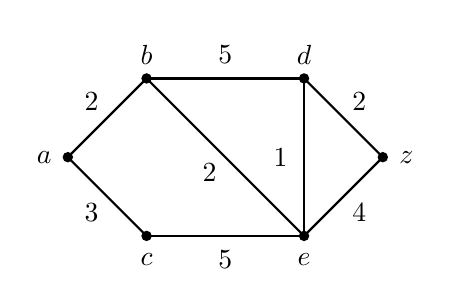
\begin{tikzpicture}
\coordinate (a) at (0,0);
\coordinate (b) at (1,1);
\coordinate (c) at (1,-1);
\coordinate (d) at (3,1);
\coordinate (e) at (3,-1);
\coordinate (z) at (4,0);
\begin{scope}[thick]
% draws vertices
\node[circle, fill=black,scale = 0.4] at (a){};
\node[circle, fill=black,scale = 0.4] at (b){};
\node[circle, fill=black,scale = 0.4] at (c){};
\node[circle, fill=black,scale = 0.4] at (d){};
\node[circle, fill=black,scale = 0.4] at (e){};
\node[circle, fill=black,scale = 0.4] at (z){};
% labels vertices
\node at (-0.3,0) {$a$};
\node at (1,1.3) {$b$};
\node at (1,-1.3) {$c$};
\node at (3,1.3) {$d$};
\node at (3,-1.3) {$e$};
\node at (4.3,0) {$z$};
% draws edges
\draw[postaction={decorate}] (a) to (b);
\draw[postaction={decorate}] (b) to (d);
\draw[postaction={decorate}] (d) to (z);
\draw[postaction={decorate}] (z) to (e);
\draw[postaction={decorate}] (e) to (c);
\draw[postaction={decorate}] (c) to (a);
\draw[postaction={decorate}] (b) to (e);
\draw[postaction={decorate}] (d) to (e);
% labels edges
\node at (0.3,0.7) {$2$};
\node at (0.3,-0.7) {$3$};
\node at (2,1.3) {$5$};
\node at (2,-1.3) {$5$};
\node at (1.8,-0.2) {$2$};
\node at (2.7,0) {$1$};
\node at (3.7,0.7) {$2$};
\node at (3.7,-0.7) {$4$};
\end{scope}
\end{tikzpicture}
\end{center}
Solution:
First, set $S=\emptyset$, then, with the table below implementing Dijkstra's Algorithm, the shortest length is 7.


\end{problem}

\begin{table}[h!]
\caption{Dijkstra's Algorithm for Exercise 3}
\label{tab:table1}
\centering
\begin{tabular}{llllllll}
 step &    1    & 2         & 3         & 4        & 5         & 6  \\
 $L(a)$&    0     & 0         & 0         & 0        & 0         & 0\\
 $L(b)$& $\infty$ & 2         & 2         & 2        & 2         & 2\\
 $L(c)$& $\infty$ & $\infty$  & 3         & 3        & 3         & 3\\
 $L(d)$& $\infty$ & $\infty$  & $\infty$  & $\infty$ & 5         & 5\\
 $L(e)$& $\infty$ & $\infty$  & $\infty$  & 4        & 4         & 4\\
 $L(z)$& $\infty$ & $\infty$  & $\infty$  & $\infty$ & $\infty$  & 7\\
 $S$   & $\{a\}$  & $\{a,b\}$ & $\{a,b,c\}$  & $\{a,b,c,e\}$  & $\{a,b,c,e,d\}$  &$\{a,b,c,e,d,z\}$ \\
 
\end{tabular}
\end{table}
\begin{problem}{\S 10.6 - 5}
Find a shortest path between $a$ and $z$ in the weighted graph in Exercise~3.

Solution:
By Dijkstra's Algorithm, the shortest path between $a$ and $z$ is
$\{a,b,e,d,z\}$
\end{problem}
\begin{problem}{\S 10.6 - 6}
Find the length of a shortest path between these pairs of
vertices in the weighted graph in Exercise 3.
\begin{enumerate}
\item[(a)] $a$ and $d$
\item[(d)] $b$ and $z$
\end{enumerate}
By Dijkstra's Algorithm, the length of the shortest path between $a$ and $d$ is 5.
By Dijkstra's Algorithm, the length of the shortest path between $b$ and $z$ is 5.
\end{problem}
\begin{problem}{\S 10.6 - 7}
Find shortest paths in the weighted graph in Exercise 3
between the pairs of vertices in Exercise 6 (parts a and d).

Solution:

By Dijkstra's Algorithm, the shortest path between $a$ and $d$ is
$\{a,b,e,d\}$
\end{problem}
\begin{problem}{\S 10.6 - 26}
Solve the traveling salesperson problem for this graph
by finding the total weight of all Hamilton circuits and
determining a circuit with minimum total weight.
\begin{center}
\begin{tikzpicture}
\coordinate (a) at (1,2);
\coordinate (b) at (3,2);
\coordinate (c) at (4,0);
\coordinate (d) at (2,-1);
\coordinate (e) at (0,0);
\begin{scope}[thick]
% draws vertices
\node[circle, fill=black,scale = 0.4] at (a){};
\node[circle, fill=black,scale = 0.4] at (b){};
\node[circle, fill=black,scale = 0.4] at (c){};
\node[circle, fill=black,scale = 0.4] at (d){};
\node[circle, fill=black,scale = 0.4] at (e){};
\node[circle, fill=black,scale = 0.4] at (z){};
% labels vertices
\node at (0.8,2.2) {$a$};
\node at (3.2,2.2) {$b$};
\node at (4.3,0) {$c$};
\node at (2,-1.3) {$d$};
\node at (-0.3,0) {$e$};
% draws edges
\draw[postaction={decorate}] (a) to (b);
\draw[postaction={decorate}] (a) to (c);
\draw[postaction={decorate}] (a) to (d);
\draw[postaction={decorate}] (a) to (e);
\draw[postaction={decorate}] (b) to (c);
\draw[postaction={decorate}] (b) to (d);
\draw[postaction={decorate}] (b) to (e);
\draw[postaction={decorate}] (c) to (d);
\draw[postaction={decorate}] (c) to (e);
\draw[postaction={decorate}] (d) to (e);
% labels edges
\node at (0.3,1) {$7$};
\node at (2,2.2) {$3$};
\node at (3.7,1) {$10$};
\node at (3,-0.7) {$6$};
\node at (1,-0.7) {$1$};
\node at (1,0.2) {$5$};
\node at (0.9,0.8) {$2$};
\node at (3.1,0.8) {$8$};
\node at (1.7,0.5) {$4$};
\node at (2.3,0.5) {$9$};
\end{scope}
\end{tikzpicture}
\end{center}
Solution:
The minimum total weight will be 20, due to my enumerate below.

\end{problem}
\begin{table}[h!]
\caption{10.6-28 Solution table}
\label{tab:table2}
\centering
\begin{tabular}{llllllll}
 Circuit & Weight    \\
 a-b-c-d-e-a&3 +10+6+1+7=27\\
 a-b-c-e-d-a&3 +10+5+1+4=23\\
 a-b-d-c-e-a&3 +9+6+5+7=30\\
 a-b-d-e-c-a&3 +9+1+5+8=26\\
 a-b-e-c-d-a&3 +2+5+6+4=20\\
 a-b-e-d-c-a&3 +2+1+6+8=20\\
 a-c-b-d-e-a&8 +10+9+1+7=35\\
 a-c-b-e-d-a&8 +10+2+1+4=25\\
 a-c-d-b-e-a&8 +6+9+2+7=32\\
 a-c-e-b-d-a&8 +5+2+9+4=28\\
 a-d-b-c-e-a&4 +9+10+5+7=35\\
 a-d-c-b-e-a&4 +6+10+2+7=29
       
\end{tabular}
\end{table}
\begin{problem}{\S 10.7 - 6}
Determine whether the given graph is planar.
If so, draw it so that no edges cross.
\begin{center}
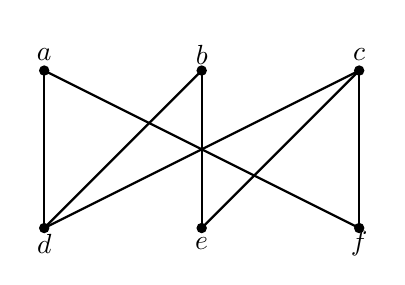
\begin{tikzpicture}
\coordinate (a) at (0,2);
\coordinate (b) at (2,2);
\coordinate (c) at (4,2);
\coordinate (d) at (0,0);
\coordinate (e) at (2,0);
\coordinate (f) at (4,0);
\begin{scope}[thick]
% draws vertices
\node[circle, fill=black,scale = 0.4] at (a){};
\node[circle, fill=black,scale = 0.4] at (b){};
\node[circle, fill=black,scale = 0.4] at (c){};
\node[circle, fill=black,scale = 0.4] at (d){};
\node[circle, fill=black,scale = 0.4] at (e){};
\node[circle, fill=black,scale = 0.4] at (f){};
% labels vertices
\node at (0,2.2) {$a$};
\node at (2,2.2) {$b$};
\node at (4,2.2) {$c$};
\node at (0,-0.2) {$d$};
\node at (2,-0.2) {$e$};
\node at (4,-0.2) {$f$};
% draws edges
\draw[postaction={decorate}] (a) to (d);
\draw[postaction={decorate}] (a) to (f);
\draw[postaction={decorate}] (b) to (d);
\draw[postaction={decorate}] (b) to (e);
\draw[postaction={decorate}] (c) to (d);
\draw[postaction={decorate}] (c) to (e);
\draw[postaction={decorate}] (c) to (f);
\end{scope}
\end{tikzpicture}
\end{center}
Solution:

It is a planar graph,
\begin{center}
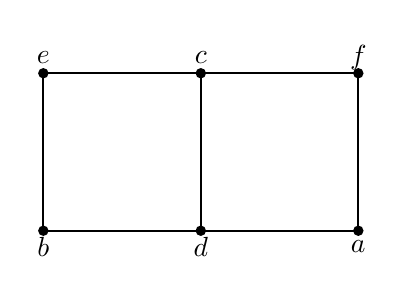
\begin{tikzpicture}
\coordinate (a) at (0,2);
\coordinate (b) at (2,2);
\coordinate (c) at (4,2);
\coordinate (d) at (0,0);
\coordinate (e) at (2,0);
\coordinate (f) at (4,0);
\begin{scope}[thick]
% draws vertices
\node[circle, fill=black,scale = 0.4] at (a){};
\node[circle, fill=black,scale = 0.4] at (b){};
\node[circle, fill=black,scale = 0.4] at (c){};
\node[circle, fill=black,scale = 0.4] at (d){};
\node[circle, fill=black,scale = 0.4] at (e){};
\node[circle, fill=black,scale = 0.4] at (f){};
% labels vertices
\node at (0,2.2) {$e$};
\node at (2,2.2) {$c$};
\node at (4,2.2) {$f$};
\node at (0,-0.2) {$b$};
\node at (2,-0.2) {$d$};
\node at (4,-0.2) {$a$};
% draws edges
\draw[postaction={decorate}] (a) to (b);
\draw[postaction={decorate}] (a) to (d);
\draw[postaction={decorate}] (b) to (e);
\draw[postaction={decorate}] (b) to (c);
\draw[postaction={decorate}] (c) to (f);
\draw[postaction={decorate}] (d) to (e);
\draw[postaction={decorate}] (e) to (f);
\end{scope}
\end{tikzpicture}
\end{center}
\end{problem}
\begin{problem}{\S 10.7 - 11}
Show that $K_5$ is nonplanar using an argument similar to that given in Example 3.

Solution:
Since $K_5$ is fully connected between any pair of vertices, there must be an edge between $v_1$ and $v_2$, $v_2$ and $v_3$, $v_3$ and $v_4$, $v_1$ and $v_4$, $v_1$ and $v_3$, $v_4$ and $v_2$, which seperates the space into two spaces, and $v_2$ is inside the circuit, but $v_5$ is outside, so it is impossible to connect them without intersection with other edges.  

\end{problem}
\begin{figure}[h!]
    \centering
    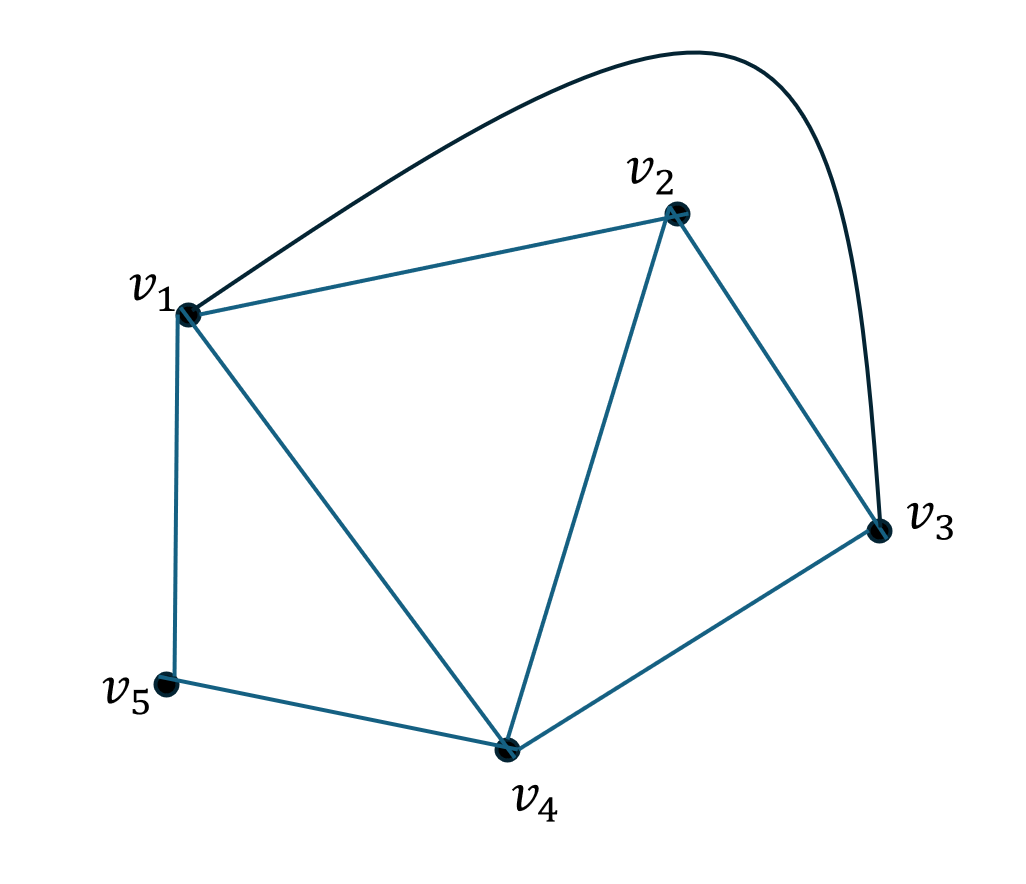
\includegraphics[width=0.5\linewidth]{屏幕截图 2024-12-03 175057.png}
    \caption{Graph for 10.7-11}
    \label{fig:enter-label}
\end{figure}
\begin{problem}{\S 10.7 - 13}
Suppose that a connected planar graph has six vertices, each of degree four. Into
how many regions is the plane divided by a planar representation of this graph?

Solution:

There are 7 seperated space by this graph.
\end{problem}
\begin{figure}[h!]
    \centering
    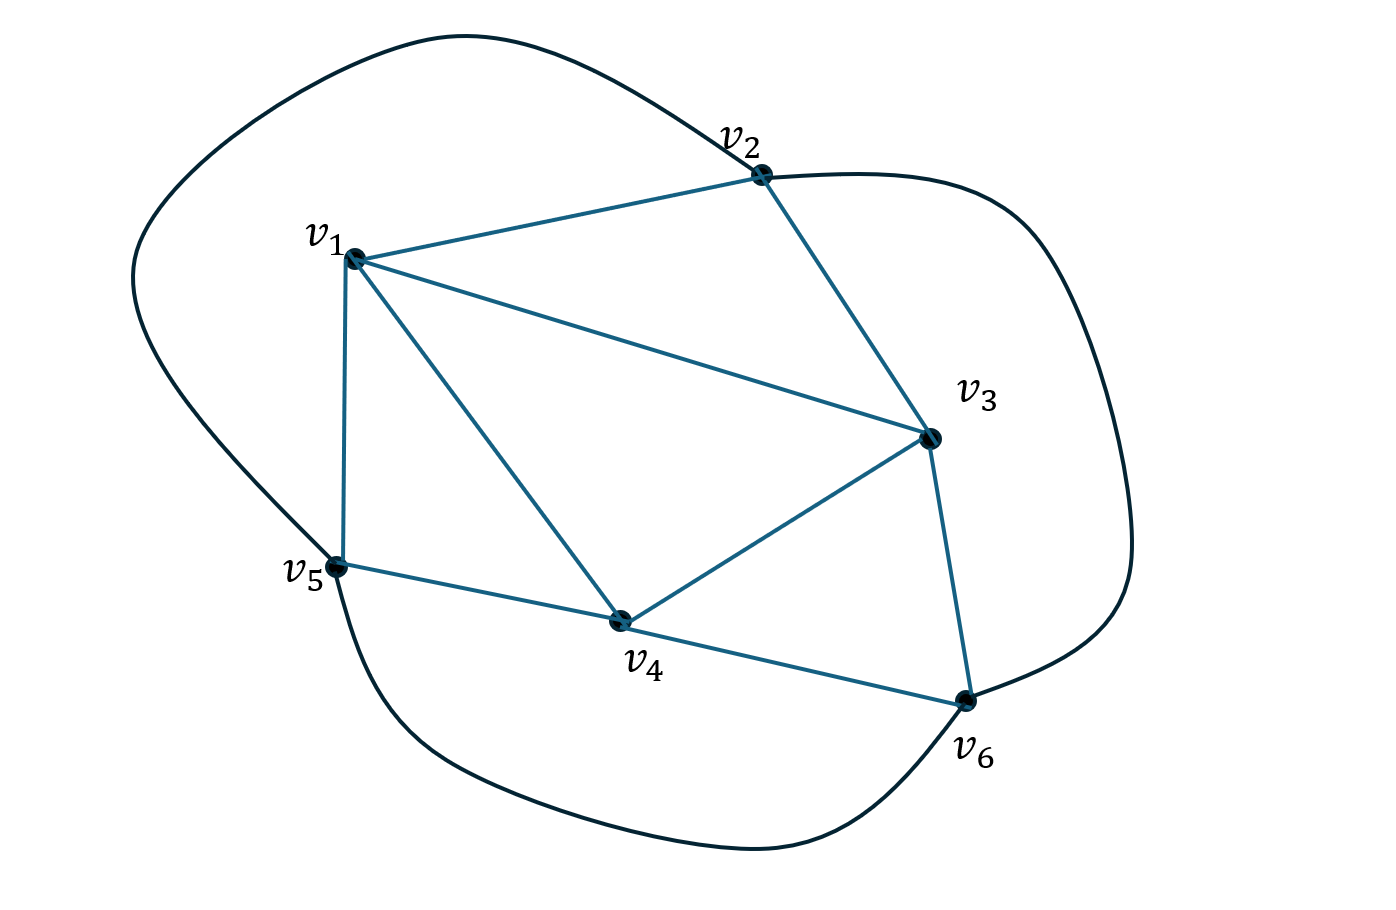
\includegraphics[width=0.5\linewidth]{屏幕截图 2024-12-03 180426.png}
    \caption{Graph for 10.7-13}
    \label{fig:enter-label}
\end{figure}
\begin{problem}{\S 10.7 - 14}
Suppose that a connected planar graph has $30$ edges. If a planar representation of
this graph divides the plane into $20$ regions, how many vertices does this graph
have?

Solution:

By Eurler Formula, $r=e-v+2$, then, $20=30-v+2$, then, $v=12$, Thus, 12 vertices.
\end{problem}
\begin{problem}{\S 10.8 - 1}
Construct the dual graph for the map shown. (See Rosen for the map!) Then find the
number of colors needed to color the map so that no two adjacent regions have the
same color.

Solution:
The graph is below in Figure 3, and the number of colors needed to color the map to meet the requirement is $4$
\end{problem}
\begin{figure}[h!]
    \centering
    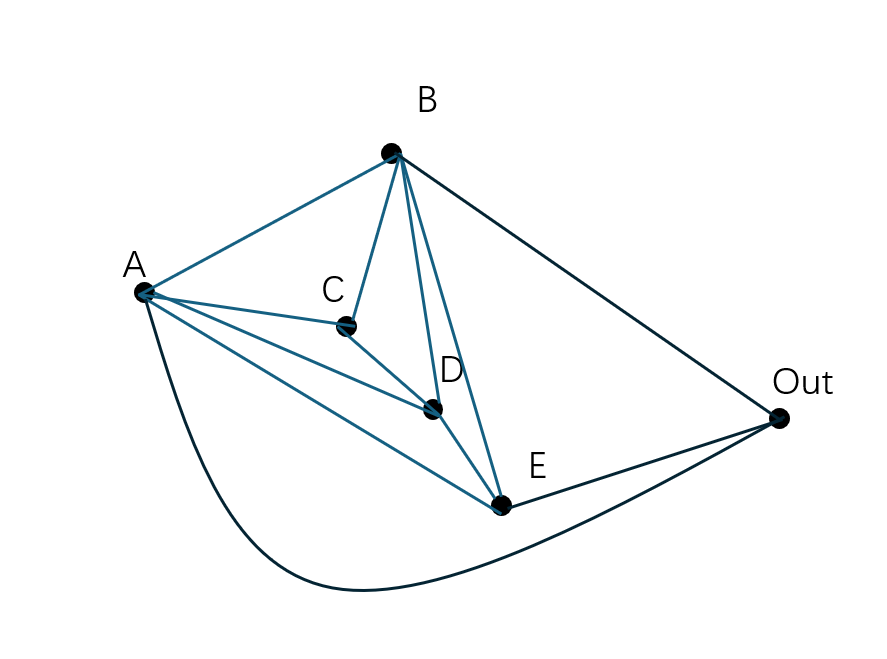
\includegraphics[width=0.5\linewidth]{屏幕截图 2024-12-04 121927.png}
    \caption{10.8-1 Graph}
    \label{fig:enter-label}
\end{figure}

\begin{problem}{\S 10.8 - 5}
Find the chromatic number of the given graph.
\begin{center}
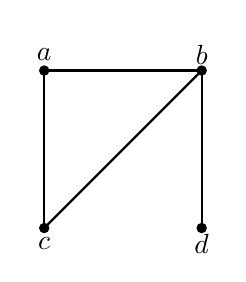
\begin{tikzpicture}
\coordinate (a) at (0,2);
\coordinate (b) at (2,2);
\coordinate (c) at (0,0);
\coordinate (d) at (2,0);
\begin{scope}[thick]
% draws vertices
\node[circle, fill=black,scale = 0.4] at (a){};
\node[circle, fill=black,scale = 0.4] at (b){};
\node[circle, fill=black,scale = 0.4] at (c){};
\node[circle, fill=black,scale = 0.4] at (d){};
% labels vertices
\node at (0,2.2) {$a$};
\node at (2,2.2) {$b$};
\node at (0,-0.2) {$c$};
\node at (2,-0.2) {$d$};
% draws edges
\draw[postaction={decorate}] (a) to (b);
\draw[postaction={decorate}] (a) to (c);
\draw[postaction={decorate}] (b) to (c);
\draw[postaction={decorate}] (b) to (d);
\end{scope}
\end{tikzpicture}
\end{center}
Solution:

The chromatic number of this graph is $3$ since $a$ and $b$ are adjacent, they should have different color, $b$ and $c$ are adjacent, they should have different color, and $a$ and $c$ are adjacent, so different color. Thus, there are $3$ colors, but for $d$, since it only adjacent with $b$, it can be same color as $a$ or $c$, thus still $3$.
\end{problem}
\begin{problem}{\S 10.8 - 6}
Find the chromatic number of the given graph.
\begin{center}
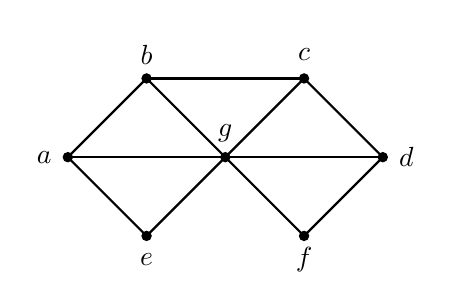
\begin{tikzpicture}
\coordinate (a) at (0,0);
\coordinate (b) at (1,1);
\coordinate (c) at (3,1);
\coordinate (d) at (4,0);
\coordinate (e) at (3,-1);
\coordinate (f) at (1,-1);
\coordinate (g) at (2,0);
\begin{scope}[thick]
% draws vertices
\node[circle, fill=black,scale = 0.4] at (a){};
\node[circle, fill=black,scale = 0.4] at (b){};
\node[circle, fill=black,scale = 0.4] at (c){};
\node[circle, fill=black,scale = 0.4] at (d){};
\node[circle, fill=black,scale = 0.4] at (e){};
\node[circle, fill=black,scale = 0.4] at (f){};
\node[circle, fill=black,scale = 0.4] at (g){};
% labels vertices
\node at (-0.3,0) {$a$};
\node at (1,1.3) {$b$};
\node at (3,1.3) {$c$};
\node at (4.3,0) {$d$};
\node at (1,-1.3) {$e$};
\node at (3,-1.3) {$f$};
\node at (2,0.3) {$g$};
% draws edges
\draw[postaction={decorate}] (a) to (b);
\draw[postaction={decorate}] (b) to (c);
\draw[postaction={decorate}] (c) to (d);
\draw[postaction={decorate}] (d) to (e);
\draw[postaction={decorate}] (f) to (a);
\draw[postaction={decorate}] (a) to (g);
\draw[postaction={decorate}] (b) to (g);
\draw[postaction={decorate}] (c) to (g);
\draw[postaction={decorate}] (d) to (g);
\draw[postaction={decorate}] (e) to (g);
\draw[postaction={decorate}] (f) to (g);
\end{scope}
\end{tikzpicture}
\end{center}
Solution:

The chromatic number of this graph is $3$ since $b$ and $c$ are adjacent, they should have different color, $b$ and $g$ are adjacent, they should have different color, and $c$ and $g$ are adjacent, so different color. Thus, there are $3$ colors, but for $d$, since it only adjacent with $c$ and $g$ which already assigned color, it can be same color as $b$. And for $a$, since only adjacent with $b$ and $g$ which already assigned color, it can be same color with $c$. and for $e$ since only adjacent with $a$ and $g$, it can be same as $b$, similarly, $f$ can be same color as $c$. So, in total, still $3$ colors.
\end{problem}
\begin{problem}{\S 10.8 - 15}
What is the chromatic number of $W_n$?

Solution:

$W_n$ is a wheel graph, thus, it is forming by $C_n$ with an vertex in the center, connecting all vertex in $C_n$. Thus, the basic structure are many triangles. for one triangle planar graph, it should contain three different color in each vertex to make no adjacent have same color. And when other points afflicated on this triangle by connecting with one center vertex and a vertex on the circle, it can have the same color with the vertex on that triangle it doesn't connected with, thus, whenever adding how many vertices, it will still be $3$ colors. But, when coming to the last edge connecting the base vertex of those triangle in two sides (The red edge in the graph below). When the vertices connected by the two graph has identical color, one of them should change to another color, which will end up with $4$ different color. Thus, in case if $n$ is odd number, the chromatic number of this graph is $4$, and if $n$ is even number, the chromatic number is $3$.
\[\begin{cases}
    3 \text{ $n$ is even number}\\
    4 \text{ $n$ is odd number}
\end{cases}\]
\end{problem}
\begin{figure}[h!]
    \centering
    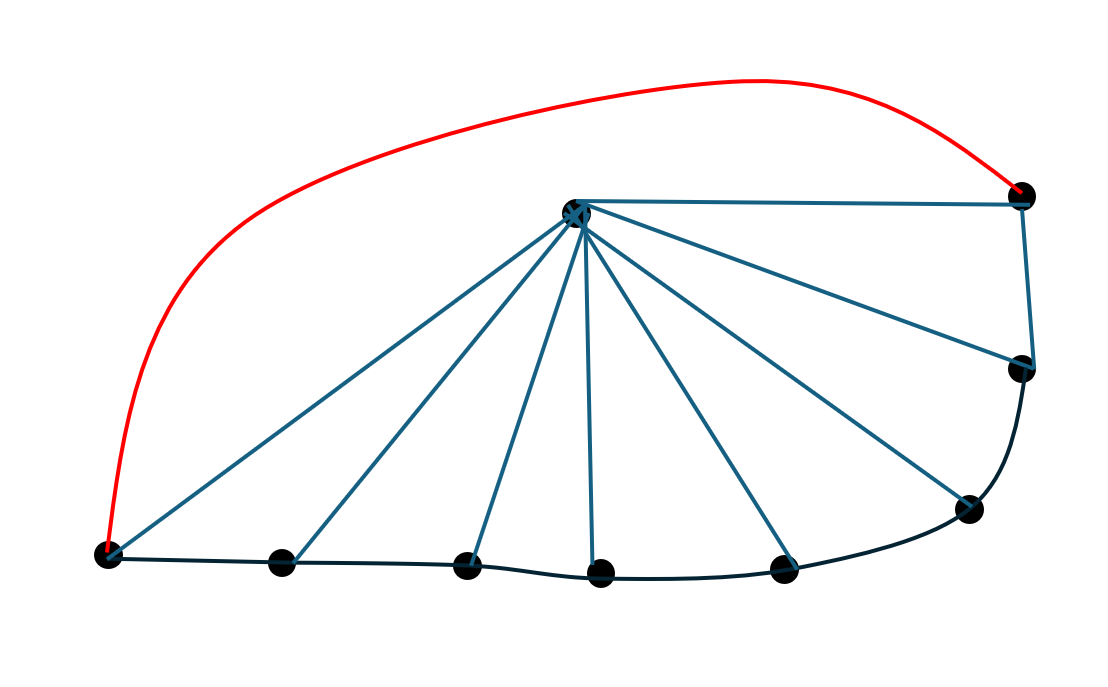
\includegraphics[width=0.5\linewidth]{屏幕截图 2024-12-04 124324.png}
    \caption{10.8-15 Graph}
    \label{fig:enter-label}
\end{figure}
\begin{problem}{\S 10.8 - 16}
Show that a simple graph that has a circuit with an odd
number of vertices in it cannot be colored using two colors.

Solution:

Suppose a simple graph with odd number of vertices forms a circuit. $v_1,\cdots,v_n$, where $n$ is odd number. Then, if we assign them in pair, which pair wise connected, like $v_1-v_2$, each pair should contain different color. but there will be an vertex that cannot form with other vertices to form a pair since odd number cannot divided by 2. Then, when we try to connect those pairs head to end, it will form a circuit with the last vertex has the two adjacent vertex with different color. Thus, this vertex should have different color with both vertices to meet the requirement. Thus, it cannot be colored using two colors.
\end{problem}
\end{document}